\documentclass{article}
\usepackage[utf8]{inputenc}
\usepackage{fullpage}
\usepackage{graphicx}
\usepackage{subfigure}
\graphicspath{ {./images/} }

\usepackage{amsmath}
\usepackage[usenames,dvipsnames]{color}
%\usepackage{soul}
\usepackage[normalem]{ulem}  %for \sout (strikeout)
\usepackage{xspace}
\newcommand{\red}[1]{{\color{red}{#1}\xspace}}


\title{Thesis Report}
\author{Isha Anantpurkar}
\date{November 2020}

\begin{document}

\maketitle

\red{To get a new paragraph, just leave a blank line in the text. That
will do the correct indenting. Don't use two backslahes. I fixed most of
them.}

\section{Introduction}
Gravitational-wave detectors such as LIGO, VIRGO, KAGRA \red{KAGRA doesn't
have any detections yet} have
detected Gravitational Waves (GWs) radiated from compact object
coalescences, such as binary black hole (BBH) systems and binary
black hole neutron star systems (NSBH) systems. The data from
these detectors \red{\sout{consists of} contain}
a large amount of noise in which the
gravitational wave signals are buried. In order to extract these
signals, the process of matched filtering is used, where a set of
template waveforms \red{\sout{are} is}
compared with the detector data. Hence, the
detection of gravitational waves depends on the template waveforms
chosen \red{\sout{to matched filter the detector data.} for the
matched filtering.}

The efficiency of the template bank in recovering signals from data
depends on the density of template waveforms in the parameter space
and the waveforms \red{\sout{itself} themselves}.
Full numerical simulations of \red{all the} waveforms
in the bank are not possible \red{\sout{due to} because of}
the computational cost of
the simulations. \red{\sout{and h} H}ence, approximants such as Post-Newtonian
(PN) and Effective One Body (EOB) formalism are used to construct
these waveforms. The use of these inexact waveforms can reduce
the detection rate of GWs. Additionally, these template waveforms
usually \red{\sout{only}} consist \red{only}
of the dominant quadrupolar mode. This \red{\sout{affects the} reduces
the likelihood of}
detection of GWs from binary systems with high mass ratios and
spin, which contain observable contributions from sub-dominant modes
(as observed in GW190814).

So, in order to detect these binary systems, it is important to
understand the waveform models most appropriate to these regions in
parameter space, \red{especially}
the effect of including higher modes in template waveforms.


\section{Gravitational Waves from Coalescing Binaries}
\begin{figure}[h]
    \centering
    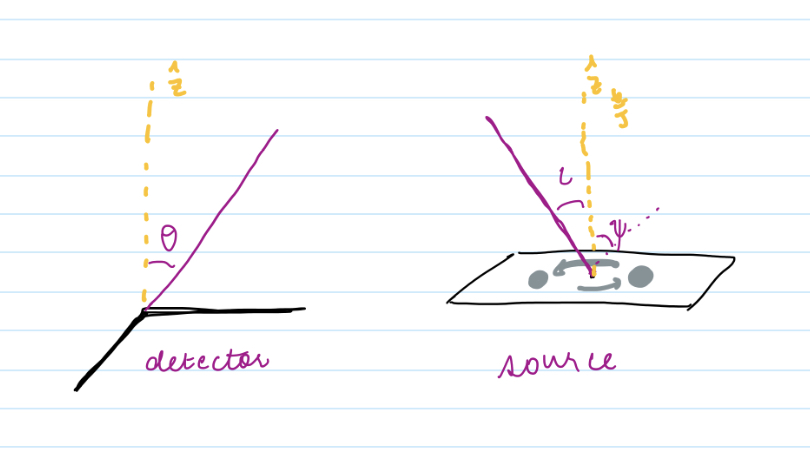
\includegraphics[scale=0.2]{params.jpeg}
    \caption{Parameters in gravitational wave detection}
    \label{fig:my_label}
\end{figure}

\red{\sout{The above image} Figure \ref{fig:my_label} (you can't count on
the figure ending up right above the current text)} shows the
source and detector frames and important angles.  The inclination
angle $\iota$ is the angle between the line connecting the detector
and source and the total angular momentum of the binary $\vec{J}$
(the polarization of the grav wave \red{I don't think this is the
polarization angle. Take a look at Figs 7 and 8 in Ch2 of Duncan Brown's
thesis}).  The angle $\phi_0$ is the
phase (coalescence phase \red{I don't think this is the coalescence phase.
It's just the phase angle in the frame of the binary. The subscript 0 is
an unfortunate choice of notation. I think a c is used for coalescence.}
) of the binary evolution and depends on the
starting point.  The angles $\theta$ and $\phi$ \red{\sout{are} give}
the position of the binary in the sky \red{in the frame of the detector}.
\red{Explain the angle $\psi$ e.g. as the 3rd Euler angle relating the
binary frame to the detector frame. Maybe you should download the source
for Brown's thesis from ArXiV and reproduce a couple of his figures?}

\red{A} gravitational waveform is represented
as a time-series function $h(t)$, where $h$ is written in terms of
the plus and cross polarizations,
\begin{equation}
    h(t) = h_{+}(t) + ih_{\times}(t). \label{ComplexTimeSeries}
\end{equation}
\red{\sout{which} This}
can be written in terms of spin-weighted spherical harmonic functions,
\begin{equation}
    h(t) = \sum_{l=2}^{\infty} \sum_{m=-l}^{l} Y^{-2}_{lm}(\iota, \phi_0) \; h_{lm}(t) \label{SpinWheighted}
\end{equation}
The $Y^{-2}_{lm}$s are functions of the inclination angle and phase.
\red{Is this right? I thought $h(t)$ was written in terms of $\theta$ and
$\phi$ in the detector frame.}
The $l=2$, $m=2$ mode corresponds to the quadrupole mode,
which is dominant in gravitational radiation.

\section{Detection of Gravitational Waves}
\subsection{Matched filtering}
The gravitational wave data from detectors can be represented as,
\begin{equation}
    d(t) = n(t) + h(t) ,\label{GWData}
\end{equation}
where $n(t)$ is the Gaussian \red{The noise is not generally Gaussian,
although over short periods in time it is often approximted as
Gaussian. Much of the analysis goes through without this assumption. Can
you make it clear where you really need the Gaussian assumption?}
background noise and $h(t)$ is the gravitational waveform signal. In order to identify these signals from the data, the data is match filtered with a set of theoretical waveforms called the template bank.

The signal-to-noise ratio (SNR) $\rho$ is used to quantify the match between two waveforms. For GW data $d(t)$ and normalized theoretical waveforms $\hat{h_b}(t)$ \red{$\hat h_b(t)$ (hat centered on $h$)},
\begin{equation}
    \rho = max_{params} \left( d(t), \hat{h_b}(t)\right), %\label{SNR}
\end{equation}
\red{
\begin{equation}
    \rho = \max_\text{params} \left( d(t), \hat h_b (t)\right), \label{SNR}
\end{equation}
By using the amsmath package (which I added), you get operators like
max that give nice spacing. Also note the use of the text macro from
amsmath to get params in the correct font.
}
where $(,)$ is the inner product defined by
\begin{equation}
    (h_1, h_2) = 4 \int_{0}^{\infty} \frac{\tilde h_1^* (f)
    \tilde h_2 (f)}{S_n(f)}df.
\end{equation}
\red{(I fixed the centering of the tildes)}
\red{\sout{and is} This quantity is to be}
maximized over all parameters of the waveform. A GW is ``detected''
\red{(In Latex, the open quote is a back tick, different from a forward 
tick (apostrophe) used for a close quote. Also, we usually use double
quotes in ordinary text.)} if the SNR is above a set minimum.

\red{\sout{However,}} The template bank \red{\sout{used cannot
consist of waveforms spanning all of the} is discrete and so
cannot encompass every waveform in the continuous} parameter
space. Additionally, the waveform approximants used to construct
the template bank may not \red{\sout{be the same as} accurately
represent} the actual waveforms from
binaries. \red{\sout{This effect} These effects}
of the discreteness of template banks and use
of waveform approximants \red{\sout{is} are}
represented by the fitting factor (FF),
\begin{equation}
    \text{FF} = \max_\text{template bank}
    \left ( \hat{h}_s(t), \hat{h}_b(t)\right ),
\end{equation}
where $h_s$ is the signal waveform and $h_b$ is the template bank waveform.
\red{Note how the text macro takes care of the correct fonts and spacing}

The fitting factor also gives us a measure of how well a template bank can recover signal waveforms, since a greater fitting factor would mean greater SNR would be recovered. This is known as the effectualness of a template bank.  

\subsection{Geometric Placement of Template Banks} \label{GeomTmplBank}
Template bank generating algorithms have the purpose of generating the minimum number of waveforms such that any waveform in that parameter space can be recovered with a fitting factor of 0.97 or higher.
{\red Explain that 0.97 is chosen so that no more than  X\% of signals
are missed.}

\red{\sout{Define} Start by defining}
\begin{equation}
    O(h_1, h_2) = \left( \hat{h}_1, \hat{h}_2\right)
\end{equation}
as the normalized overlap between two waveforms. Let $\lambda$ be a point in the parameter space and $\lambda + \Delta\lambda$ be a point very close to the first point ($\Delta\lambda \approx $ 0).
Then, the overlap for waveforms at these two points can be written as,
\begin{equation}
    O(h(\lambda), h(\lambda + \Delta\lambda)) \approx 1 + \frac{1}{2} \left (\frac{\partial^2O}{\partial\Delta\lambda^i \; \partial\Delta\lambda^j} \right) \delta\lambda^i \delta\lambda^j
\end{equation}
\red{Explain why the first-order term is zero}
where the 1 is the \red{\sout{first order} zeroth-order}
value of the overlap, for $\Delta\lambda = 0$. \red{Setting} the second term
\red{\sout{is defined as} to} $-g_{ij}\delta\lambda^i \delta\lambda^j$
\red{\sout{and} allows us to define a metric} $g_{ij}$ \red{\sout{is the
metric} that can be} used to find the points in the template bank.

\red{You need a few more sentences here explaining how you actually place
points using the metric.}

In the case where a template bank is constructed with non\red{-}spinning binary systems, the metric is represented in $\tau_0$, $\tau_3$ coordinates,
where~\cite{TmplBank}  \red{put citation in text, not inside equation}
\begin{equation}
    \tau_0 = \frac{5}{265 \pi f_0 \eta}\left(\frac{\pi G M f_0}{c^3}
    \right)^{-5/3} \qquad
     \tau_3 = \frac{5}{8 f_0 \eta} \left( \frac{\pi G M f_0}{c^3}\right)^{-2/3}.
\red{\text{Define }\eta \quad f_0}
\end{equation}
\red{Note use of quad or qquad macros for spacing in equation}
\red{\sout{because} The reason for this choice
is that} the metric is more cartesian in these coordinates.
\red{\sout{The plots below} Figure~\ref{fig:mtau}} shows a temple bank for
non-spinning binary black holes in $m_1$, $m_2$ coordinates and $\tau_0$, $\tau_3$ coordinates. The points in the $\tau_0 - \tau_3$ plot are more uniformly distributed as compared to the $m_1 - m_2$ plot.
\begin{figure}[h]
    \begin{minipage}{0.5\textwidth}
        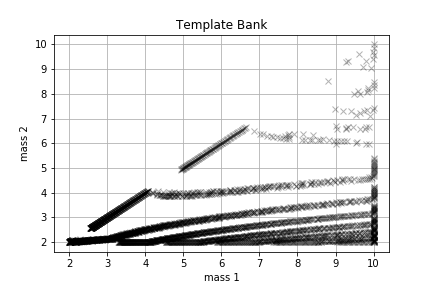
\includegraphics[scale=0.5]{m1m2.png}
        \label{fig:m1m2}
    \end{minipage}
    \begin{minipage}{0.5\textwidth}
        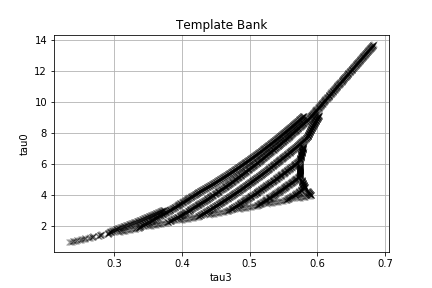
\includegraphics[scale=0.5]{tau0tau3.png}
        \label{fig:tau0tau3}
    \end{minipage}
    \caption{Template Bank for non-spinning binaries with component masses
2 -- 10 $M_{\odot}$ plotted in $m_1$-$m_2$ coordinates to the left and
$\tau_0$-$\tau_3$ coordinates to the right. \label{fig:mtau}}
\end{figure}

\subsection{Effectualness of Template Banks}

\red{We computed the}
effectualness of a template bank consisting of EOBNRv2 waveforms \red{\sout{was
found to signal} for input signals from} EOBNRv2 and TaylorF2 waveforms.
The template bank was
constructed using the method described in Section \ref{GeomTmplBank}
for non-spinning binaries with component masses $3$ -- $25\,M_{\odot}$. The
plot of fitting factors for EOBNRv2 waveform signals is shown
\red{\sout{below} in Fig.~\ref{fig:effectualnessEOB}}.
In this case, the regions with lower fitting factors reflect
the lack of template waveforms in those regions, \red{while} the points with
FF close to 1 coincide with the points in the template bank. This
is \red{\sout{more clear} clearer}
from the second plot in $\eta-\mathcal{M}$ coordinates.
\red{Define $\mathcal{M}$}
\begin{figure}[h]
    \begin{minipage}{0.5\textwidth}
        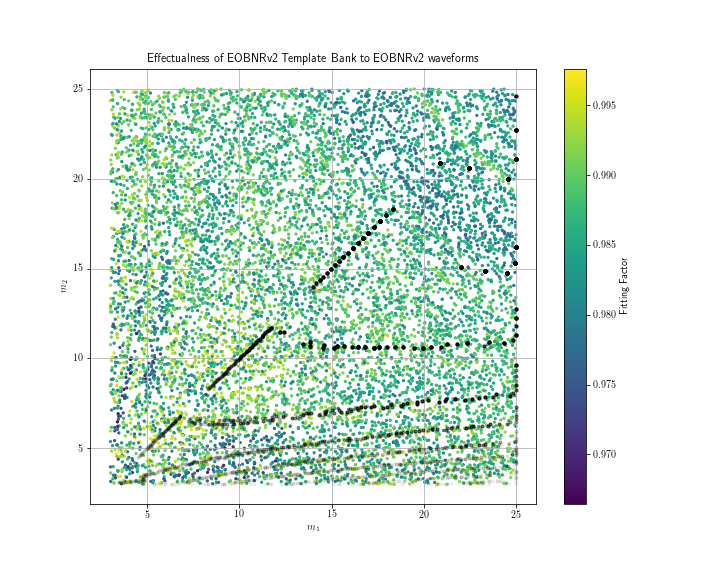
\includegraphics[scale=0.3]{EffectualnessEOBNRv2.png}
        \label{fig:effectualnessEOBm1m2}
    \end{minipage}
    \begin{minipage}{0.5\textwidth}
        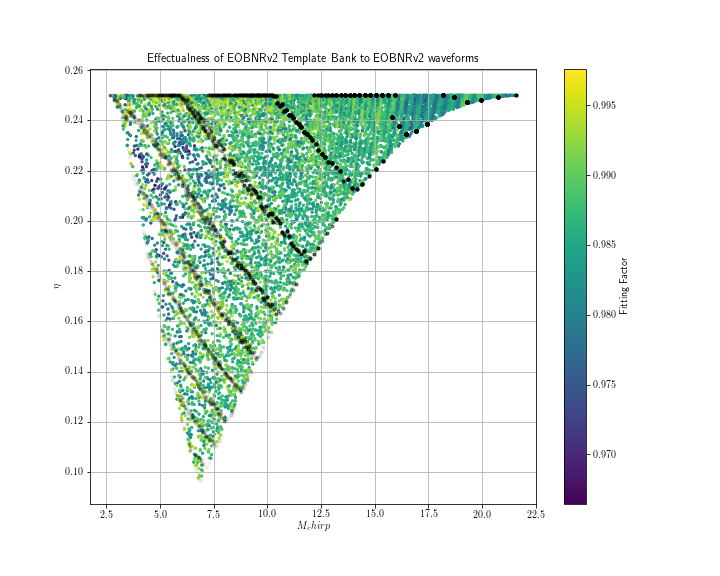
\includegraphics[scale=0.3]{EffectualnessEOBNRv2-eta-mchirp-coords.png}
        \label{fig:effectualnessEOBetamchirp}
    \end{minipage}
    \caption{Fitting Factor of EOBNRv2 signal waveforms in $m_1$-$m_2$
    coordinates and $\eta$-$\mathcal{M}$ coordinates}
    \label{fig:effectualnessEOB}
\end{figure}

\red{\sout{The plot below} Figure~\ref{fig:effectualnessTaylorF2}}
shows the FF of TaylorF2 signal waveforms. The FF
here decreases for larger total mass $M$ which could be because
the PN approximated waveforms only contain the inspiral
waveform. These waveforms have a high frequency cutoff at the ISCO
(innermost stable circular orbit) where the adiabatic approximation
is no longer valid. Since high total mass binaries have a shorter
inspiral period, this is not sufficient to approximate the waveform.
\begin{figure}[h!]
    \centering
    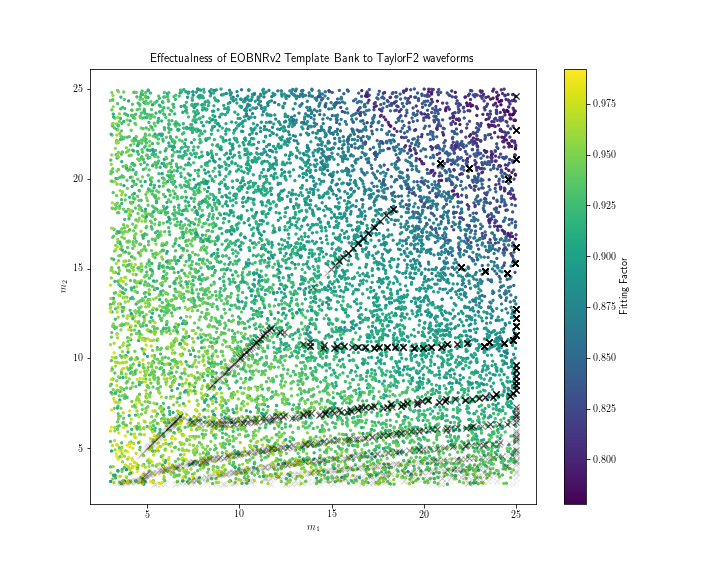
\includegraphics[scale=0.3]{EffectualnessTaylorF2.png}
    \caption{Fitting Factor of TaylorF2 signal waveforms.
    \label{fig:effectualnessTaylorF2}}
\end{figure}

For full waveforms including the merger, phenomenological models are used.
\red{\sout{which} These} are constructed using PN approximated waveforms tuned to numerical relativity for merger and ringdown terms. 


\begin{thebibliography}{1}
\bibitem{TmplBank} Babak, S. et al., Phys.Rev. D87 024033 (2013)
\end{thebibliography}

\end{document}
